\documentclass[dvipdfmx]{article}
\usepackage{tikz}
\usetikzlibrary{decorations,decorations.pathreplacing}

\begin{document}
  \begin{minipage}{0.33\hsize}
   \begin{center}
    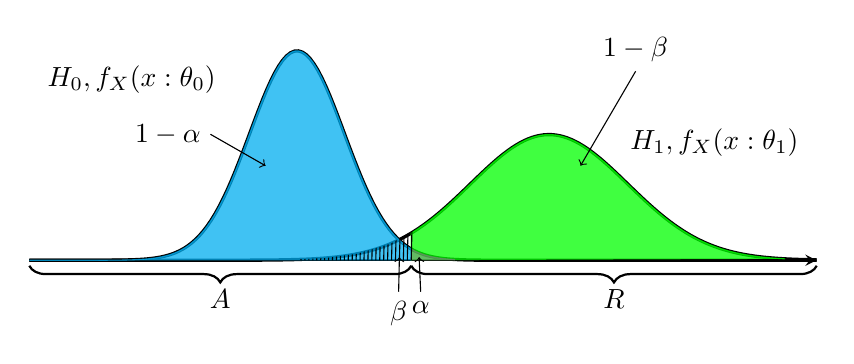
\begin{tikzpicture} [xscale = 1.0, yscale = 4]
     % 座標軸
     \draw [thick, -stealth](-5.0,0)--(5.0,0) node [anchor=north]{$$};

     % 正規分布
     \draw [very thick, domain=-5.0:5.0, samples=200] plot(\x, {exp((-(\x+1.6)^2)/(2*0.6^2))/(sqrt(2*pi*0.6^2))});
     \draw [very thick, domain=-5.0:5.0, samples=200] plot(\x, {exp((-(\x-1.6)^2)/2)/(sqrt(2*pi))});


     % 領域 塗りつぶし
     %\filldraw [green, opacity=.75, domain=-0.150:4.6, samples=200](-0.150,{exp((-(-0.150+1.6)^2)/(2*0.6^2))/(sqrt(2*pi*0.6^2))})--plot(\x, {exp((-(\x-1.6)^2)/2)/(sqrt(2*pi))})--plot(\x, {exp((-(\x+1.6)^2)/(2*0.6^2))/(sqrt(2*pi*0.6^2))});
\filldraw [green, opacity=.75, domain=-0.150:4.6, samples=200](-0.150,0)--plot(\x, {exp((-(\x-1.6)^2)/2)/(sqrt(2*pi))});
     \filldraw [cyan, opacity=.75, domain=-5.0:-0.150, samples=200](-5.0,0)--plot(\x, {exp((-(\x+1.6)^2)/(2*0.6^2))/(sqrt(2*pi*0.6^2))})--(-0.150,0);
     \filldraw [gray, opacity=.55, domain=-0.150:0.4, samples=200](-0.150,0)--plot(\x, {exp((-(\x+1.6)^2)/(2*0.6^2))/(sqrt(2*pi*0.6^2))})--(0.4,0);

     % 領域 斜線
     %\begin{scope}
     % \path[clip] plot[domain=-1.4:-0.150] ({\x},{exp((-(\x-1.6)^2)/2)/(sqrt(2*pi))}) -- cycle;
     % \foreach \t in {1,2,...,10}{
     % \path[draw] (0.15*\t, 0) -- (0.15*\t + 0.4, 1);
     % }
     %\end{scope}

     \begin{scope}
      \path[clip] plot[domain=-1.6:-0.150, samples=200] (-1.6,0) -- plot(\x, {exp((-(\x-1.6)^2)/2)/(sqrt(2*pi))}) -- (-0.150,0);
      \foreach \t in {1,2,...,29}{
      \path[draw] (0.05*\t-1.6, 0) -- (0.05*\t + 0.1 - 1.6, 1);
      }
     \end{scope}

     % 補助線
     \draw [dashed](-0.150,0) -- (-0.150, {exp((-(-0.150-1.6)^2)/2)/(sqrt(2*pi))});

     % 説明
     \node [anchor=south] at (-3.7, 0.5) {$H_0,f_X(x:\theta_0)$};
     \node [anchor=south] at (3.7, 0.3) {$H_1,f_X(x:\theta_1)$};
     \draw [thick, decorate, decoration={brace, mirror, amplitude=6pt, raise=2pt}] (-0.150,0)--(5.0,0) node [midway, yshift=-7pt,anchor=north]{$R$};
     \draw [thick, decorate, decoration={brace, mirror, amplitude=6pt, raise=2pt}] (-5.0,0)--(-0.150,0) node [midway, yshift=-7pt,anchor=north]{$A$};

     \draw[->] (-2.7, 0.4) node [anchor=east] {$1-\alpha$} -- (-2.0, 0.3);
     \draw[->] (2.7, 0.6) node [anchor=south] {$1-\beta$} -- (2.0, 0.3);
     \draw[->] (-0.310, -0.1) node [anchor=north] {$\beta$} -- (-0.30, 0.01);
     \draw[->] (-0.03, -0.1) node [anchor=north] {$\alpha$} -- (-0.05, 0.01);
    \end{tikzpicture}
   \end{center}
  \end{minipage}
\end{document}